% !TeX program = xelatex
\documentclass[12pt, a4paper]{article}

% --- Essential Packages ---
\usepackage[margin=1in]{geometry}
\usepackage{amsmath, amssymb, amsthm}
\usepackage{graphicx}
\usepackage{setspace}
\usepackage{float}
\usepackage{lastpage}
\usepackage{fontspec}
\setmainfont{Times New Roman}
\usepackage[math-style=ISO]{unicode-math}
\usepackage[table, xcdraw]{xcolor}
\usepackage[dvipsnames]{xcolor}
\usepackage{multirow}
\usepackage[framemethod=TikZ]{mdframed}
\usepackage{enumerate}
\usepackage[shortlabels]{enumitem}
\usepackage{minted}
\usepackage[linesnumbered, ruled, vlined]{algorithm2e}
\usepackage{subcaption}
\usepackage{fancyhdr}
\usepackage[colorlinks, urlbordercolor=blue]{hyperref} 

\hypersetup{
    colorlinks=true,
    linkcolor=black,
    filecolor=black,
    urlcolor=black,
}

\pagestyle{fancy}
\fancyhf{}
\fancyhead[L]{SWE 4304: Software Project Lab I}
\fancyhead[R]{Final Project Report (Group 7)}
\renewcommand{\footrulewidth}{0.4pt}
\fancyfoot[C]{Page \thepage\ of \pageref{LastPage}}

\begin{document}

\begin{titlepage}
    \begin{figure}[!h]
        \centering
        
\includegraphics[width=.2\textwidth]{images/iut_logo.png}
    \end{figure}
    \begin{center}
        \noindent\rule{\textwidth}{1.5pt}
        \Huge{\textbf{Islamic University of Technology}}\\
        \large{\textbf{Department of Computer Science and Engineering (CSE)}}\\
        \large{{B.Sc. in Software Engineering}}\\
        \vspace{0.2cm}
        \Large{\textbf{SWE 4304:} Software Project Lab I}\\
        \Large{{Winter}, 2025-2026}\\
        \noindent\rule{\textwidth}{0.5pt}

        \vspace{1cm}
        \Large{\textbf{Final Project Report}} \\
        \Large{{The ‘Drim’ Programming Language}} \\
        \vspace{1cm}

        \vspace{0.5cm}
        \large{\textbf{Group 7}} \\
        \large{Md. Muntahi Hasan Akhiar, 230042118}\\
        \large{S.M. Tahsinuzzaman Emon, 230042104}\\
        \large{Tamim Mahrush Naser, 230042133}\\

        \vspace{1.5cm}
        \large{\textbf{Supervisor}} \\
        \large{Farzana Tabassum,\\ Lecturer, CSE}\\

        \vspace{1.5cm}
        \large{{Date: March 23, 2026}} \\
    \end{center}
\end{titlepage}

\newpage
\tableofcontents
\newpage

\section{Problem Statement}
Standard programming languages can be hard for beginners because they require manual memory management and strict variable declarations. This adds a lot of extra work when someone just wants to write and run code quickly, specially beginners. 

\vspace{0.4cm}

Another problem is that most languages do not have built-in functions for things like physics formulas or unit conversions, forcing users to find and import external libraries. 

\vspace{0.4cm}

Beyond these technical issues, we also wanted to address a personal motivation. The name \textbf{“Drim”} started as an inside joke and a meme in our student batch from our first day at university. We wanted to build something that would keep this memory alive through custom keywords like \texttt{drimIn} and \texttt{drimming}. 

\vspace{0.4cm}

From an engineering perspective, we also wanted to master language design and memory management by building every component manually.

\vspace{1cm}

\section{Potential Solution}
To solve these problems, a new interpreted language called ``Drim'' was created. It is designed to be simple and easy to use for beginners. \textbf{Drim} is a custom-built, lightweight language that runs as a Command Line Interface (CLI) tool. It uses a \textbf{Tree-Walk Interpreter}, which means it reads \texttt{.drim} files, understands the code, and runs it directly in real-time. Everything in Drim was built from scratch using \textbf{C++ 17} to ensure full control over the language pipeline.

\vspace{0.4cm}

In Drim, variables are created automatically when they are first used or assigned a value, and their types are handled by the language. The language includes built-in functions for physics calculations and unit conversions so that users don't have to worry about external libraries. To keep the code safe and reliable, the interpreter uses a system where function arguments are kept strictly inside their own local space. This ensures that even during recursion, variables do not interfere with each other.

\newpage

\section{Implemented Features}
The project includes a complete system for reading, parsing, and running code. The flow of the language follows a standard interpreter pipeline, including a Lexer (Tokenizer), a Parser that builds an Abstract Syntax Tree (AST), and an Interpreter to execute the logic.


The following features were implemented:
\begin{itemize}
    \item \textbf{Input/Output:} Accepts user input through the \texttt{drim()} (input) command and shows output using \texttt{wake()} (output).
    \item \textbf{Automatic Variable Assignment:} If a value is assigned to a variable that hasn't been created yet, the system automatically creates it with the correct type.
    \item \textbf{Dynamic Type Casting:} Variables can hold different types like Strings, Integers, or Booleans, and the system handles the conversion automatically.
    \item \textbf{Data Structures Library:} Built-in support for fundamental data structures, including \textbf{Stacks} and \textbf{Queues}, for advanced data management.
    \item \textbf{High-Precision Calculations:} Implementation of \textbf{int64} support for larger integer calculations and increased internal precision.
    \item \textbf{Mathematical Operations:} Full support for arithmetic including addition (+), subtraction (-), multiplication (*), division (/), modulo (\%), and power ($\wedge$).
    \item \textbf{Bitwise Operations:} Supports bitwise AND (\&), OR ($|$), NOT ($\sim$), and bit-shifting (<<, >>) for low-level data manipulation.
    \item \textbf{Comparison \& Logical Operators:} Full set of comparison operators ($<, >, <=, >=, ==, !=$) and logical operators (\texttt{and}, \texttt{or}) for complex decision making.
    \item \textbf{Built-in Physics Functions:} Direct support for formulas like mass-energy ($E=mc^2$), force ($F=ma$), and more.
    \item \textbf{Unit Conversion Engine:} Built-in tools to convert between things like inches and centimeters, Fahrenheit and Celsius, or kilometers and feet.
    \item \textbf{Control Flow:} Supports conditional logic (if-else), loops (\texttt{drimming}), and loop control using \texttt{stopdrim} (break) and \texttt{drimagain} (continue).
    \item \textbf{Custom Syntax:} Uses unique keywords like \texttt{drimming} for loops and \texttt{wakeOut} for output to match the project's theme.
    \item \textbf{String Interpolation:} Allows variables to be put directly inside strings (like \texttt{"Value: \{x\}"}) for easier printing.
    \item \textbf{Error Reporting:} Provides clear error messages with exact locations when something goes wrong in the code.
    \item \textbf{Commenting System:} Supports single-line comments using \texttt{//}.
    \item \textbf{Headless Execution:} Runs as a lightweight tool in the terminal without needing a complex interface.
    \item \textbf{Multi-Assignment:} Allows assigning values to multiple variables at once using commas.
    \item \textbf{Arrays:} Supports array data structures for storing lists of homogeneous values and performing operations on them. 
    \item \textbf{Type Checking:} Built-in support for identifying variable types at runtime using the \texttt{type()} keyword.
    \item \textbf{Scoped Variables:} Ensures variables stay within the block where they were created.
    \item \textbf{User-Defined Functions:} Users can create their own functions that run during the program.
    \item \textbf{Recursion Support:} The language can handle functions that call themselves, allowing for more complex programming patterns.
\end{itemize}

\vspace{1cm}

\section{System Architecture Flow}
\begin{figure}[!h]
    \centering
    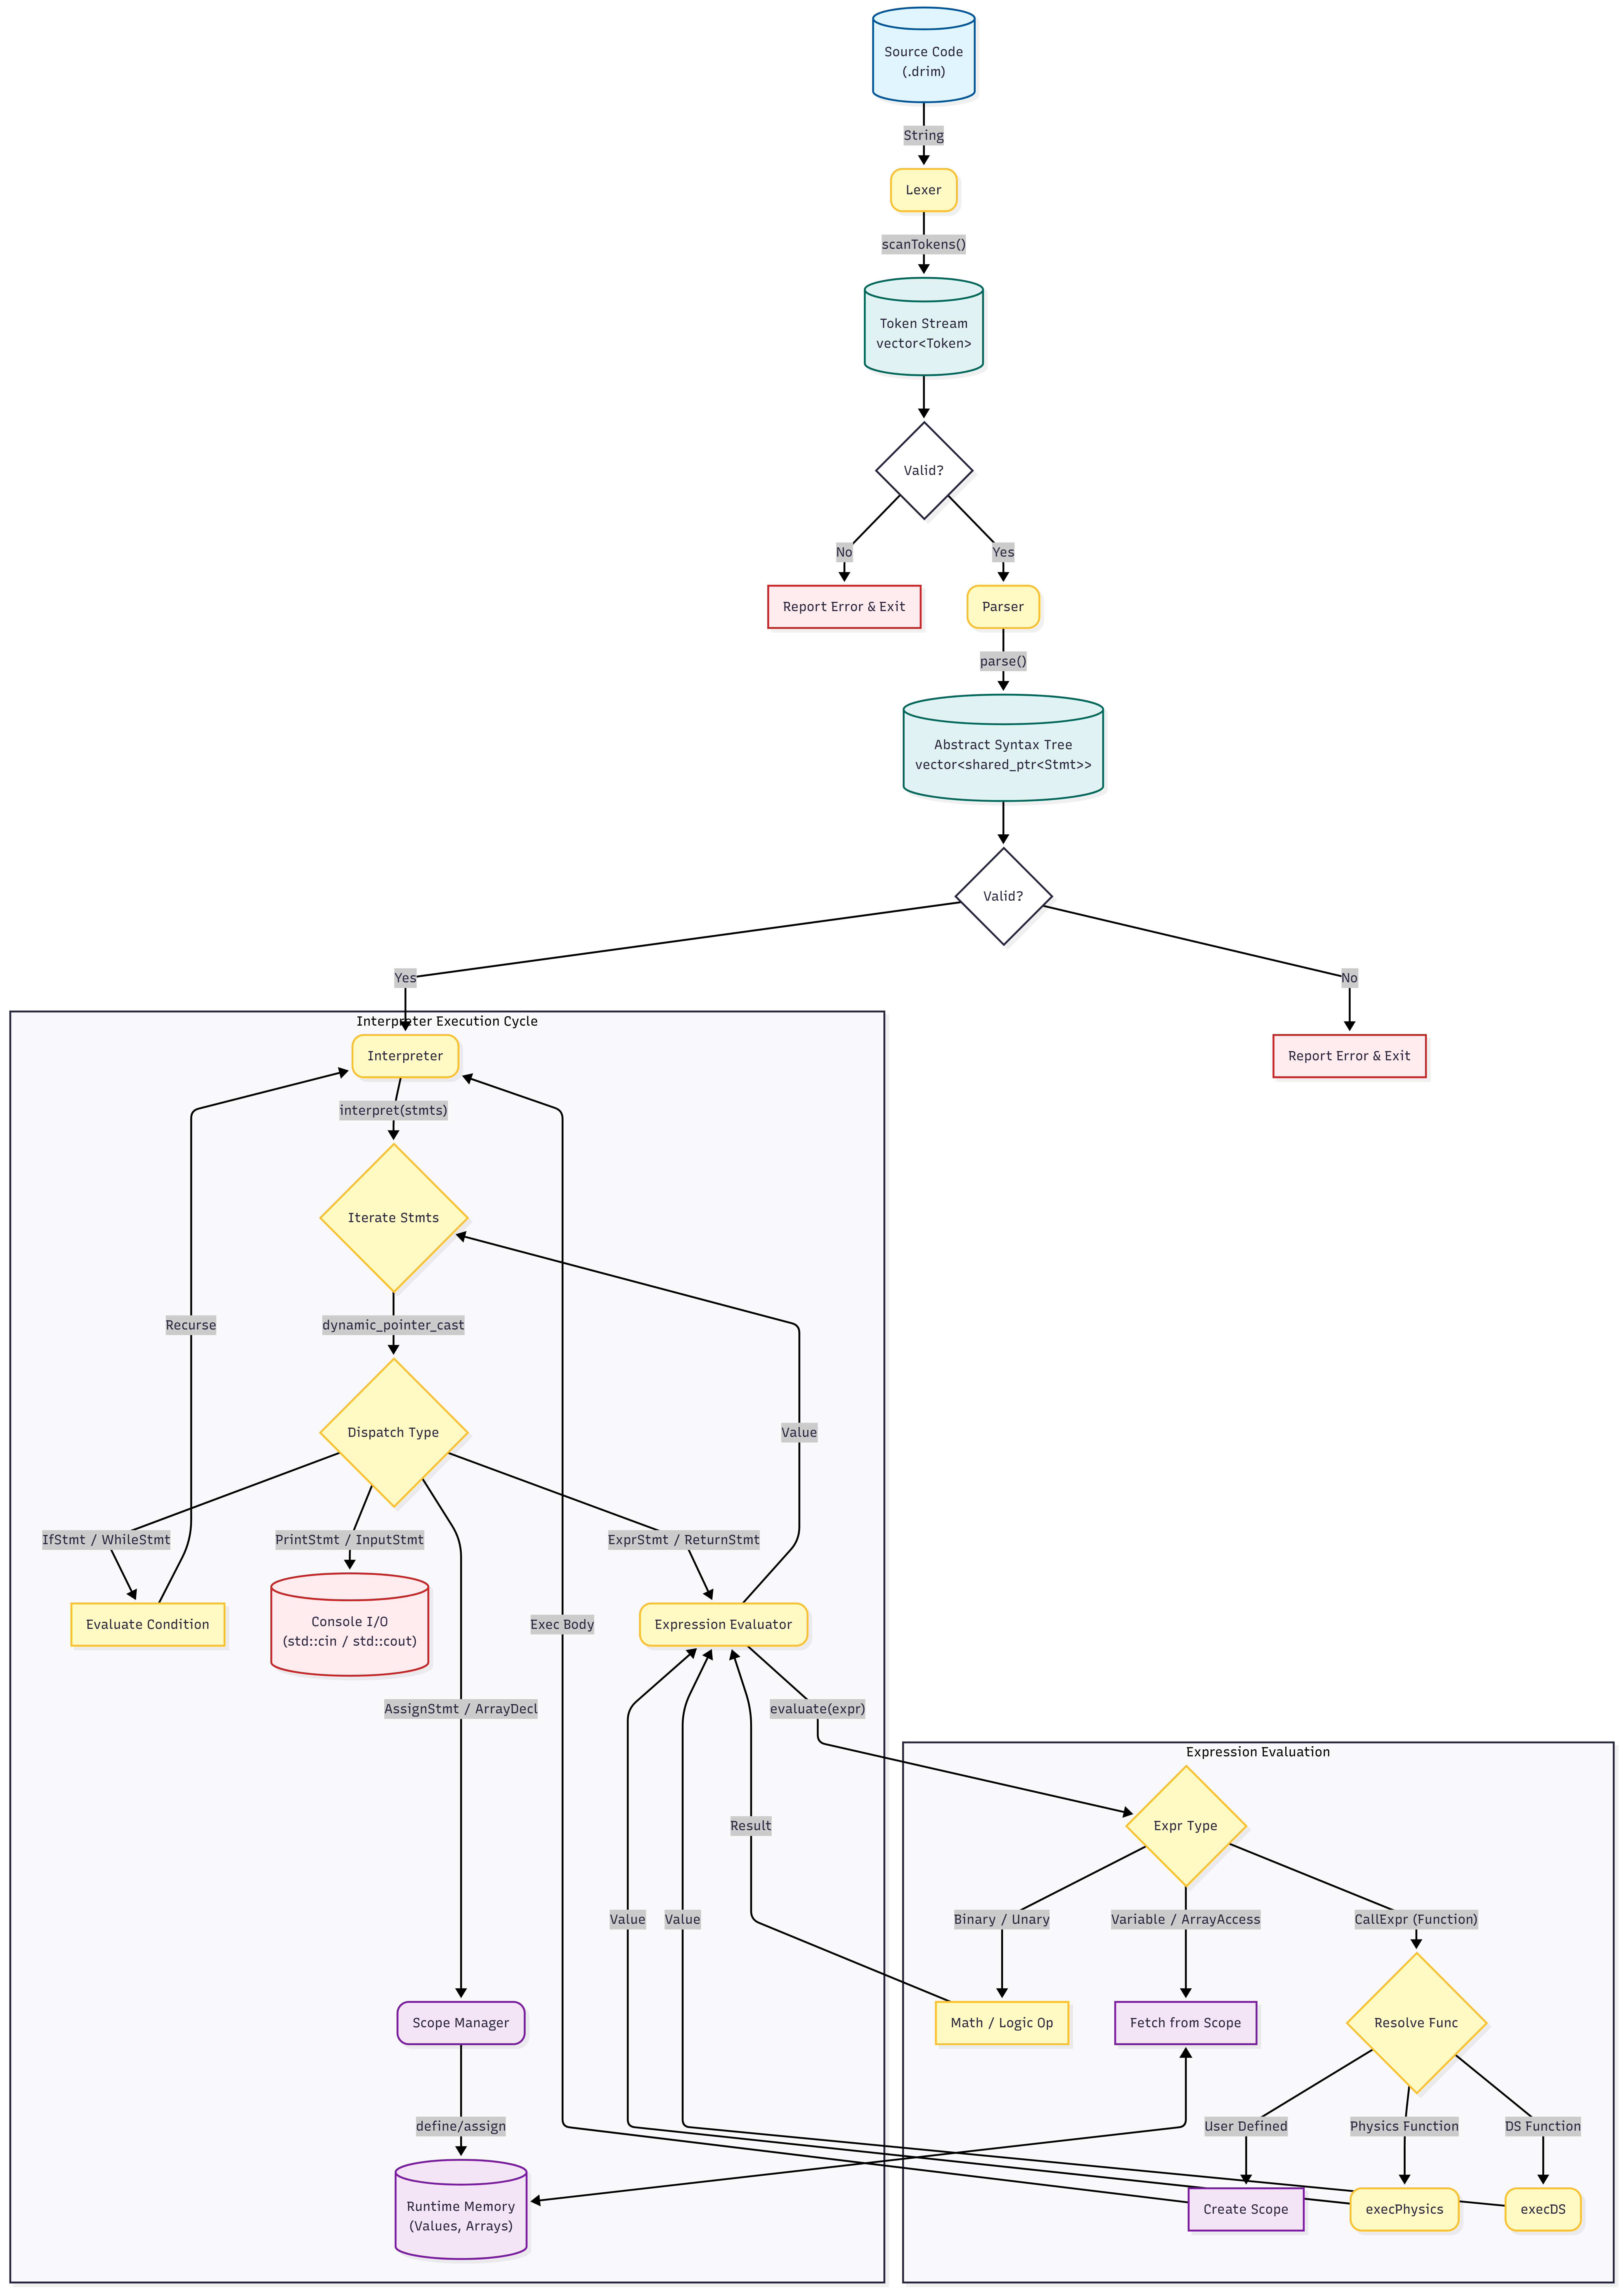
\includegraphics[width=1\linewidth]{images/FlowChartHierarchical.png}
    \caption{System Architecture Flow: From Source Code to Execution}
\end{figure}

Drim's architecture is based on a classic Tree-Walk Interpreter design. The process kicks off with the source code (\texttt{.drim} file) being read as raw text and passed to the \textbf{Lexer}. The lexer scans through the characters to group them into \textbf{Tokens} like keywords, identifiers, and operators. These tokens then move on to the \textbf{Parser}, which follows the language's grammar to build an \textbf{Abstract Syntax Tree (AST)}. This tree serves as a structural map of the entire program's logic. Finally, the \textbf{Interpreter} walks through the AST node by node, executing commands while managing variables and functions through a \textbf{Scope} system. It also hooks into specialized modules like the Physics and Data Structures engines whenever the code calls for them.

\newpage

\section{Class Diagram}
\begin{figure}[!h]
    \centering
    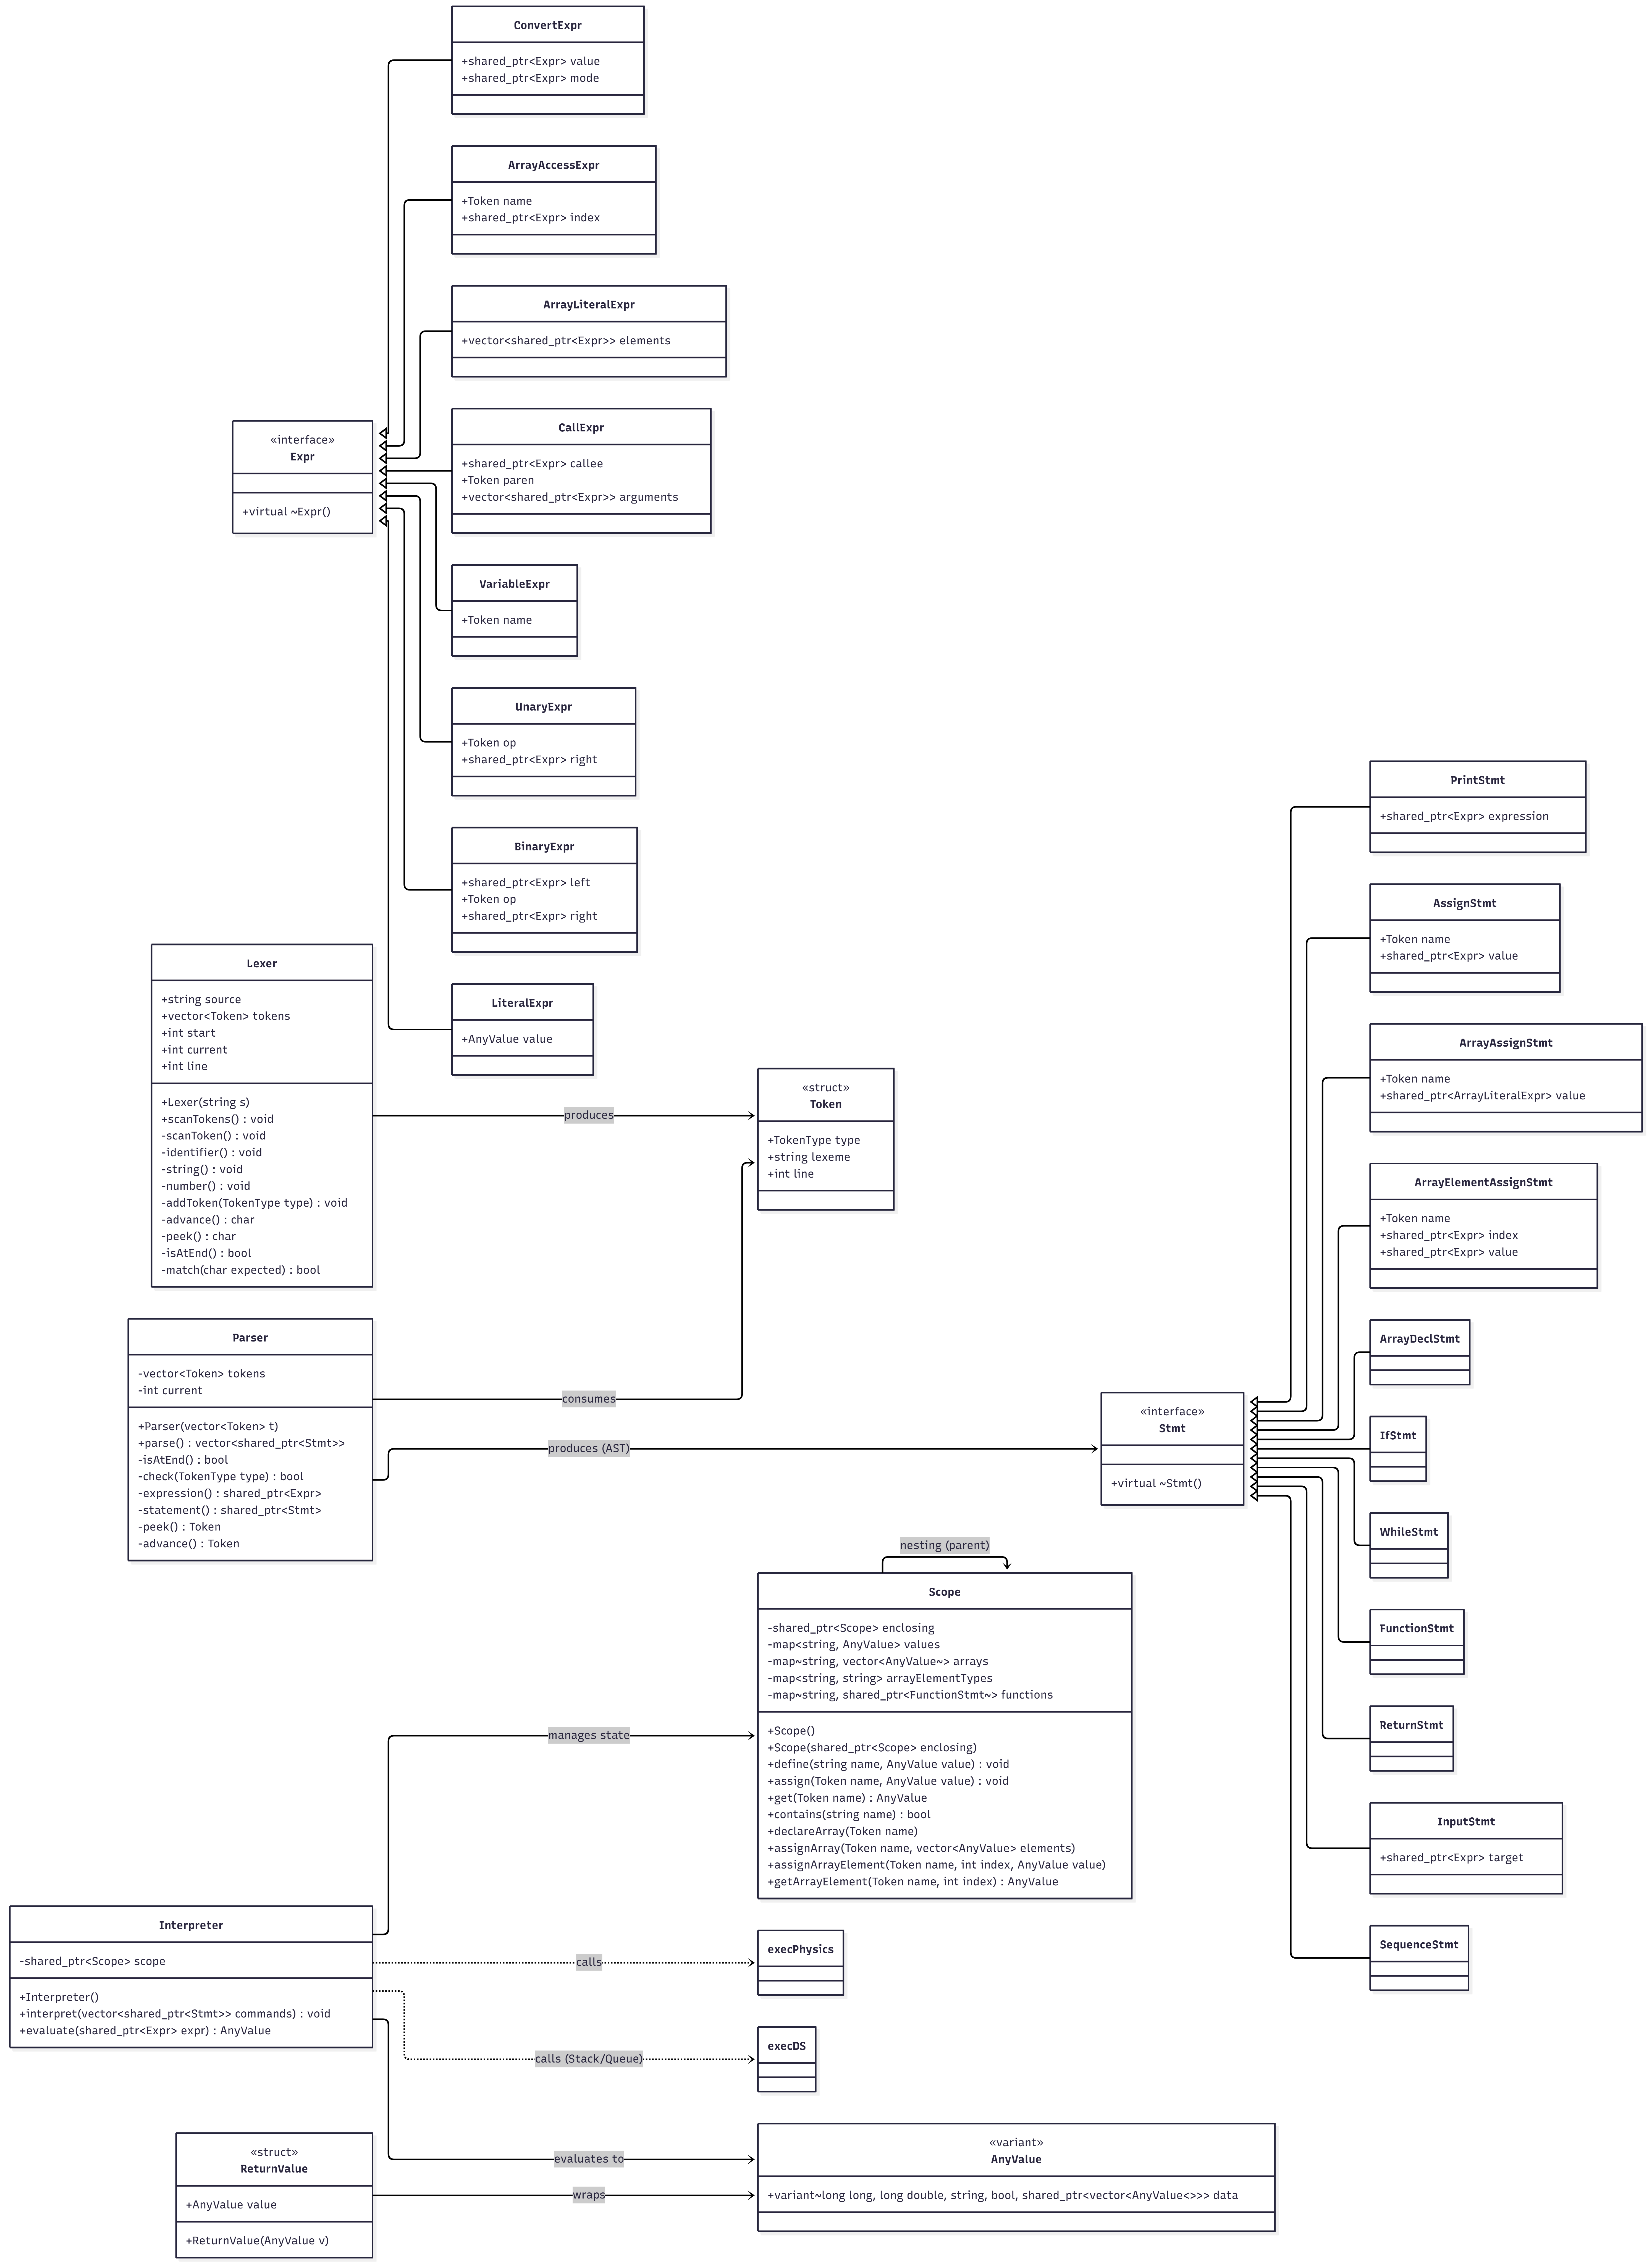
\includegraphics[width=1\linewidth]{images/FinalClassDiagramAdaptive.png}
    \caption{Project Class Diagram}
\end{figure}

The class diagram shows how Drim is structured under the hood using object-oriented principles. The language's syntax revolves around two main base structures: \texttt{Expr} (Expressions) for things that result in values, and \texttt{Stmt} (Statements) for actions. Various specific nodes, such as \texttt{BinaryExpr} for math or \texttt{IfStmt} for control flow, inherit from these bases. The \texttt{Interpreter} acts as the central engine that evaluates these nodes, relying heavily on the \texttt{Scope} class to handle memory, nested blocks, and user-defined functions. Other utility modules like the \texttt{Lexer}, \texttt{Parser}, and specialized libraries (\texttt{Physics}, \texttt{DS}) integrate into this core structure, keeping the architecture modular and decoupled.

\vspace{1cm}

\section{Design Principles}
The development of Drim was guided by the \textbf{SOLID} principles of object-oriented design to ensure the codebase remains maintainable and scalable:

\begin{itemize}
    \item \textbf{Single Responsibility Principle (SRP):} Each core component is dedicated to a specific task. The \texttt{Lexer} is responsible solely for tokenization, and the \texttt{Interpreter} for logic execution. This separation ensures that changes to the grammar do not affect the execution engine.
    \item \textbf{Liskov Substitution Principle (LSP):} The Abstract Syntax Tree (AST) is built on a hierarchy where every specific expression (e.g., \texttt{BinaryExpr}, \texttt{LiteralExpr}) can be treated as a base \texttt{Expr} object. This allows the interpreter to process any node in the tree uniformly.
    \item \textbf{Dependency Inversion Principle (DIP):} High-level execution logic in the \texttt{Interpreter} depends on abstract \texttt{Expr} and \texttt{Stmt} classes rather than concrete implementations. This decoupling allows for the easy addition of new language features without modifying the core execution loop.
\end{itemize}

\vspace{1cm}

\section{Tools and Technology}
The project used the following tools:
\begin{itemize}
    \item \textbf{Programming Language:} C++ (Standard 17) for manual control and performance.
    \item \textbf{Build System:} CMake for managing the project and making it work on different systems.
    \item \textbf{Version Control:} Git and GitHub for working together and tracking changes.
    \item \textbf{IDE:} CLion and Visual Studio Code for writing and debugging the code.
    \item \textbf{Diagrams:} Mermaid.js and Gamma for creating charts and architecture maps.
\end{itemize}

\newpage

\section{Application Domain}
The project belongs to the domain of \textbf{Custom Programming Language Design}. It is built to learn about how an interpreter actually works and to provide a specialized tool for people who need quick calculations for physics and general unit conversions. For those who want to start programming without worrying about complex syntax and memory management, Drim offers a simple and user-friendly environment.

\vspace{1cm}

\section{Project Timeline}
The project was built in stages, starting with simple text reading and moving to complex features like functions and loops.
\begin{figure}[!h]
    \centering
    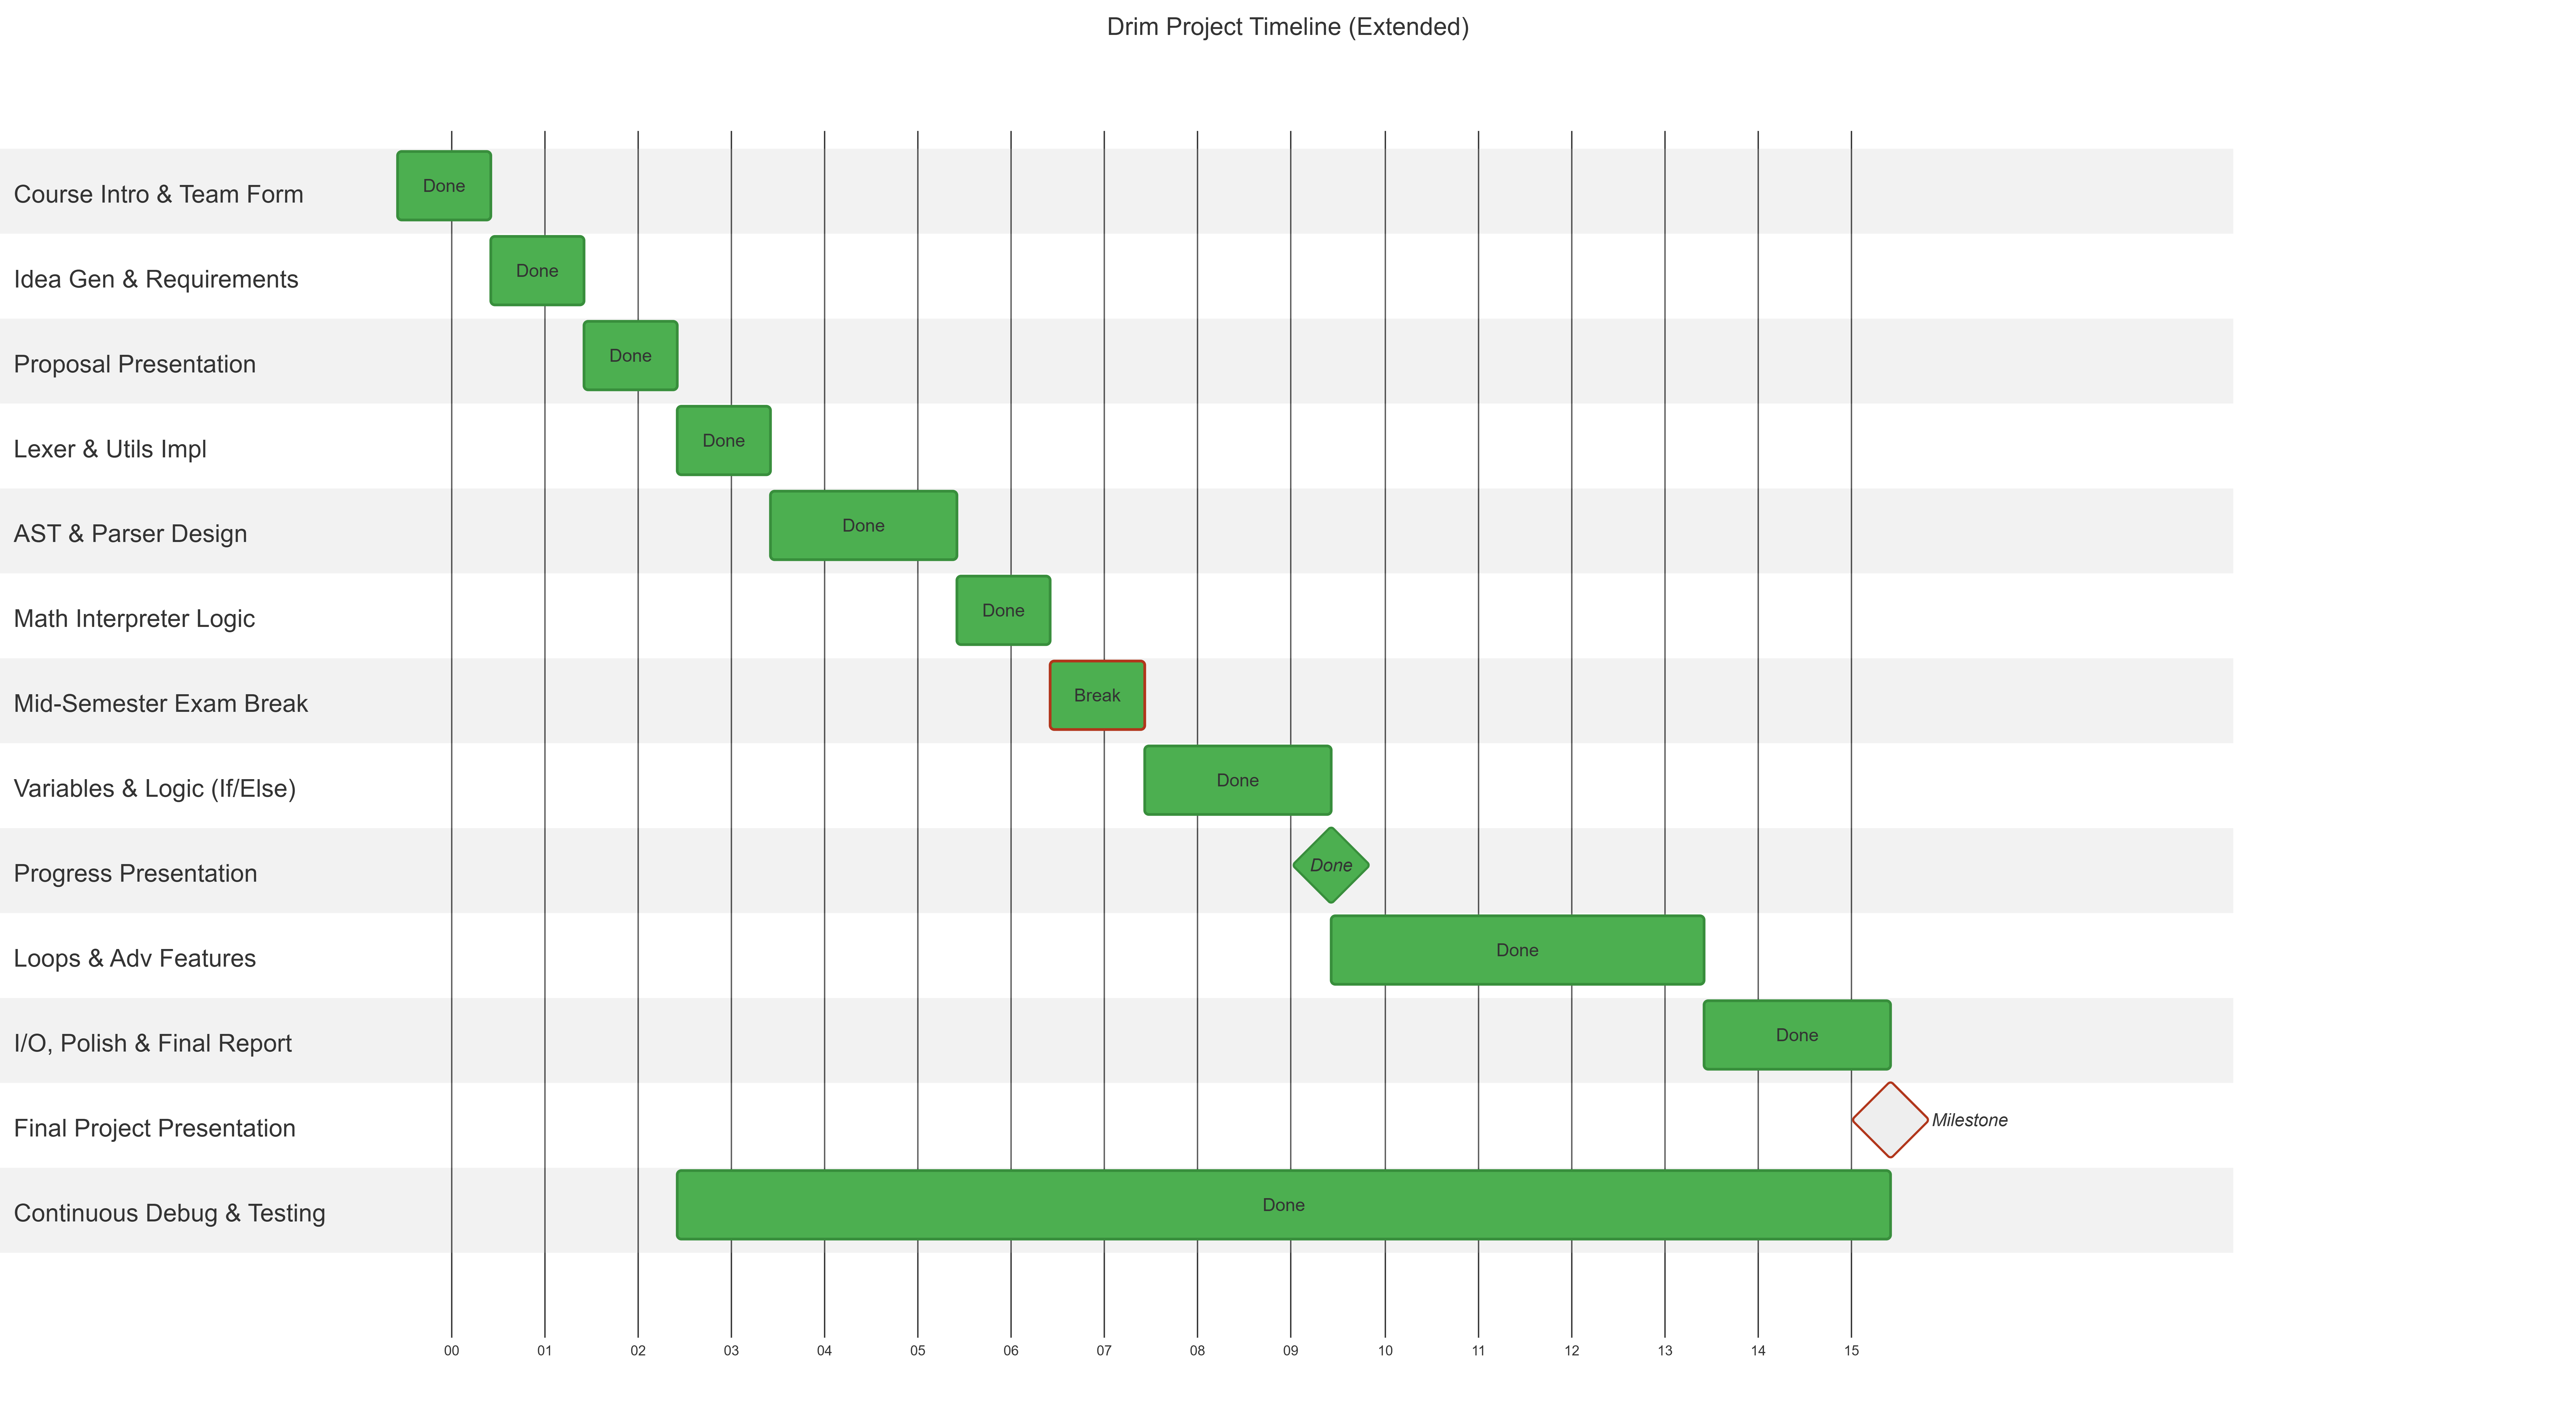
\includegraphics[width=1\linewidth]{images/Timeline.png}
    \caption{Project Development Timeline}
\end{figure}

\newpage

\section{Contribution}
The work was divided among the team members as follows:
\begin{itemize}
    \item \textbf{Md. Muntahi Hasan Akhiar:}
    \begin{itemize}
        \item Created basic input and output systems and basic architecure of lexer, parser, and interpreter with Error Reporting.
        \item Implemented variable management and automatic type casting.
        \item Developed conditional logic and loops (\texttt{drimming}).
        \item Added support for arrays and multi-assignment syntax.
        \item Added modulo operations for math.
    \end{itemize}
    \item \textbf{S.M. Tahsinuzzaman Emon:}
    \begin{itemize}
        \item Implemented mathematical operations.
        \item Built the physics function engine.
        \item Added the Boolean data type.
        \item Developed scoped variable logic.
        \item Created the system for user-defined runtime functions.
        \item Implemented String Interpolation.
    \end{itemize}
    \item \textbf{Tamim Mahrush Naser:}
    \begin{itemize}
        \item Added unit conversion functions.
        \item Worked on increasing internal calculation precision (int64).
        \item Developed a Data Structures library (Stacks, Queues, etc.).
    \end{itemize}
\end{itemize}

\vspace{1cm}

\section{Future Work}
We plan to keep improving Drim by adding more features. This includes adding many more functions for physics and unit conversions to make the language more useful. We also want to refine the core system and expand the built-in \textbf{Data Structures library} with more advanced types like Linked Lists and Trees. Other students have already started contributing on their forks, such as adding color highlighting for keywords, which we might include in the future.

\vspace{1cm}

\section{Source Repository}
The code is available at: \\
\url{https://github.com/hasanakhiar/drim-lang}

\end{document}
